\section{Auswertung}
\label{sec:Auswertung}
\subsection{Bestimmung der Zeitkonstante durch die Entladung eines Kondensators}
Die aus der mit dem Oszilloskop aufgenommenen Entladekurve des Kondensators
entnommenen Wertepaare sind in Tabelle \ref{tab:entladung} zu finden.

\begin{table}
\centering
\caption{Messdaten zur Entladung des Kondensators über den Widerstand}
\label{tab:entladung}
\begin{tabular}{c c}
\toprule
$U_\text{C}(t)/$mV & $t/$ms \\
\midrule
1088 &  0   \\
 560 &  0.5 \\
 304 &  1   \\
 152 &  1.5 \\
 80  &  2   \\
 36  &  2.5 \\
  8  &  3   \\
  4  &  3.5 \\
  2  &  4   \\
\bottomrule
\end{tabular}
\end{table}
Nach Teilen durch $U_\text{C}(0)$ und Logarithmieren von \eqref{eqn:kondensatorurelax} folgt
\begin{equation}
  \ln{\left(\frac{U_\mathrm{C}(t)}{U_0}\right)} = -\frac{t}{\tau}\,.
\end{equation}
Die graphische Darstellung der Messwerte und die Ausgleichsgerade ist in Abbildung \ref{fig:entladung}
zu sehen.
\begin{figure}
  \centering
  \includegraphics{build/uc.pdf}
  \caption{Graph von $U_\text{C}$ gegen $t$ und Ausgleichsfunktion}
  \label{fig:entladung}
\end{figure}
Die Ausgleichsgerade folgt allgemein \eqref{eqn:gerade}, sodass die Steigung der
Ausgleichsgerade $a$ mit der Zeitkonstanten $\tau$ des RC-Gliedes in dem Zusammenhang
$a = -\frac{1}{\tau}$ steht. Hier lässt sich $a$ zu
\begin{align}
  a = \SI{-1.62(007)}{\per\milli\second}
\end{align}
berechnen und für $\tau$ folgt dann
\begin{align}
\tau = RC = \SI{0.616(0027)e-3}{\second}\,.
\end{align}
\subsection{Bestimmung der Zeitkonstante durch Beachtung von Frequenzabhängigkeiten}

Die Messdaten für die eingestellte Frequenz $f$, die Kondensatorspannung
$U_\text{C}$ und die Differenz $a$ zwischen den Nulldurchgängen von Generatorspannung
und Kondensatorspannung können Tabelle \ref{tab:frequenzen} entnommen werden. Es wurde auch bereits
die Phasenverschiebung $\varphi$ aus $a$ und $f$ gemäß XXXXXXXXXXXXXXXXXXXXXXXXXXXXXXXXXXXXX berechnet.

\begin{table}
\centering
\caption{Messdaten zur Frequenzabhängigkeit der Kondensatorspannung und der Phasenverschiebung}
\label{tab:frequenzen}
\begin{tabular}{c c c c}
\toprule
$f/Hz$ & $U_\text{C}(f)/$mV & $a/$ms & $\varphi/$grad\\
\midrule
  20	&  492.30  &  1.12  &   8.06 \\
  30	&  490.85  &  1.00  &  10.80 \\
  40	&  487.05  &  0.92  &  13.25 \\
  50	&  482.15  &  0.80  &  14.40 \\
  60	&  475.17  &  0.78  &  16.85 \\
  70	&  469.05  &  0.78  &  19.56 \\
  80	&  461.20  &  0.76  &  21.89 \\
  90	&  452.80  &  0.75  &  24.36 \\
 100	&  442.15  &  0.74  &  26.78 \\
 150	&  393.80  &  0.68  &  36.72 \\
 200	&  347.30  &  0.62  &  44.93 \\
 300	&  273.00  &  0.54  &  57.89 \\
 400	&  220.20  &  0.46  &  65.66 \\
 500	&  183.00  &  0.38  &  68.40 \\
 600	&  155.70  &  0.33  &  71.71 \\
 700	&  135.60  &  0.3   &  74.59 \\
 800	&  119.80  &  0.27  &  77.18 \\
 900	&  107.30  &  0.24  &  77.76 \\
1000	&   97.00  &  0.22  &  79.20 \\
1500	&   65.50  &  0.15  &  83.16 \\
2000	&   49.35  &  0.12  &  84.96 \\
3000	&   33.06  &  0.08  &  86.40 \\
4000	&   24.88  &  0.06  &  86.40 \\
5000	&   19.96  &  0.05  &  89.28 \\
\bottomrule
\end{tabular}
\end{table}

\subsubsection{Analyse der Frequenzabhängigkeit der Kondensatorspannung}

Nach \eqref{eqn:kondensatorfrequenz} ist die Amplitude der Kondensatorspannung
$A(f) = U_\text{C}(f)$ frequenzabhängig. Es wird eine nicht lineare Ausgleichsrechnung
einer normierten Amplitude $A(f)/U_0$ mit der frequenzunabhängigen Generatorspannung $U_0$
durchgeführt. Dabei gilt für die Ausgleichsfunktion
\begin{align}
  \frac{A(f)}{U_0} = \frac{1}{\sqrt{1+d(2\pi*f)^2}}
\end{align}
 die Auftragung der Messwerte und der Graph der Ausgleichsfunktion ist in


\subsection{Der RC-Kreis als Integrator}

Für hohe angelegte Frequenzen sollte der RC-Kreis die angelegte Spannung integrieren.
Das bedeutet, dass der Graph der am Kondensator gemessenen Spannung dem Graphen der
Stammfunktion der angelegten Generatorspannung entsprechen sollte. In diesem Versuchsteil
wurde für alle angelegten Spannungen die Frequenz $f=191.8$ kHz gewählt.
Die erste an den RC-Kreis angelegte Spannung ist eine Reckteckspannung. Die Stammfunktion
zu dieser sollte gleichmäßig ansteigende Flanken dort haben, wo die Rechteckspannung
positiv ist und gleichmäßig abfallende Flanken dort, wo die Rechteckspannung
negativ ist. Es gilt der Zusammenhang
\begin{align}
  f(x)&=
  \begin{cases}
    c & 0<x\leq a\\
    -c & a<x\leq 2a
  \end{cases}
  & F(x)&=
  \begin{cases}
    c x & 0<x\leq a\\
    -c x & a<x\leq 2a
  \end{cases}
\end{align}
Genau dieses Verhalten ist in \ref{fig:rechteck} zu sehen. Der blaue Graph beschreibt
dabei die an das RC-Glied angelegte Spannung und der gelbe Graph die am Kondensator
abgegriffene Spannung.
\begin{figure}
  \centering
  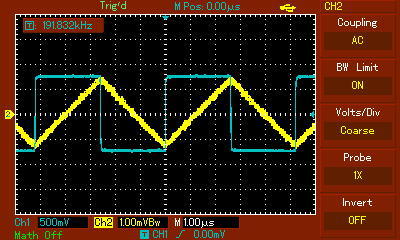
\includegraphics[width=250pt]{data/integration_rechteck.PNG}
  \caption{Graphen der Generatorspannung und der Spannung am Kondensator bei anglegter
  Rechteckspannung}
  \label{fig:rechteck}
\end{figure}


Wird an das RC-Glied eine Sägezahnspannung angelegt, so sollte die am Kondensator
abgegriffene Spannung eine sich periodisch wiederholende Funktion beschreiben, die
Extrema an den Nullstellen sowie Wendepunkten an den Extrema des Graphen der
Generatorspannung besitzt. Es gilt
\begin{align}
  f(x)&=
  \begin{cases}
    c x & -a<x\leq a\\
    -c x & a<x\leq 3a
  \end{cases}
  & F(x)&=
  \begin{cases}
    \frac{c}{2} x^2 & -a<x\leq a\\
    -\frac{c}{2} x^2 & a<x\leq 3a
  \end{cases}
\end{align}
Die Graphen der Messung \ref{fig:saegezahn} erfüllen diesen Zusammenhang.
Der blaue Graph beschreibt erneut den Verlauf der angelegten Generatorspannung und
der gelbe Graph den Verlauf der am Kondensator abgegriffenen Spannung.
\begin{figure}
  \centering
  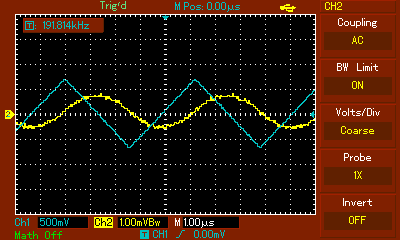
\includegraphics[width=250pt]{data/integration_saegezahn.PNG}
  \caption{Graphen der Generatorspannung und der Spannung am Kondensator bei anglegter
  Sägezahnspannung}
  \label{fig:saegezahn}
\end{figure}


Wird an den RC-Kreis eine sinusförmige Spannung angelegt, so sollte sich nach bei der
Integration gemäß
\begin{equation}
  \int c\sin(t) \, \symup{d}t=-c\cos(t) + D
\end{equation}
eine Spannung ergeben, die dem Graphen von $-\cos(t)$ entspricht. Dabei ist $c$ eine
beliebige Konstante und $D$ die Integrationskonstante. Der Verlauf der
im Versuch aufgenommenen Graphen \ref{fig:sinus} folgt dieser Beziehung. Hier beschreibt der blaue Graph
wieder den Verlauf der angelegten Generatorspannung und der gelbe Graph den Verlauf der
am Kondensator abgegriffenen Spannung.
\begin{figure}
  \centering
  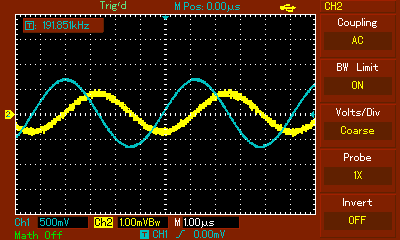
\includegraphics[width=250pt]{data/integration_sinus.PNG}
  \caption{Graphen der Generatorspannung und der Spannung am Kondensator bei anglegter
  Sinusspannung}
  \label{fig:sinus}
\end{figure}
